\documentclass[tikz,border=3pt]{standalone}
\usepackage{tikz}
\usetikzlibrary{arrows.meta,positioning,shapes.geometric,calc}
\usepackage{amsmath,amssymb}

\begin{document}
\sffamily
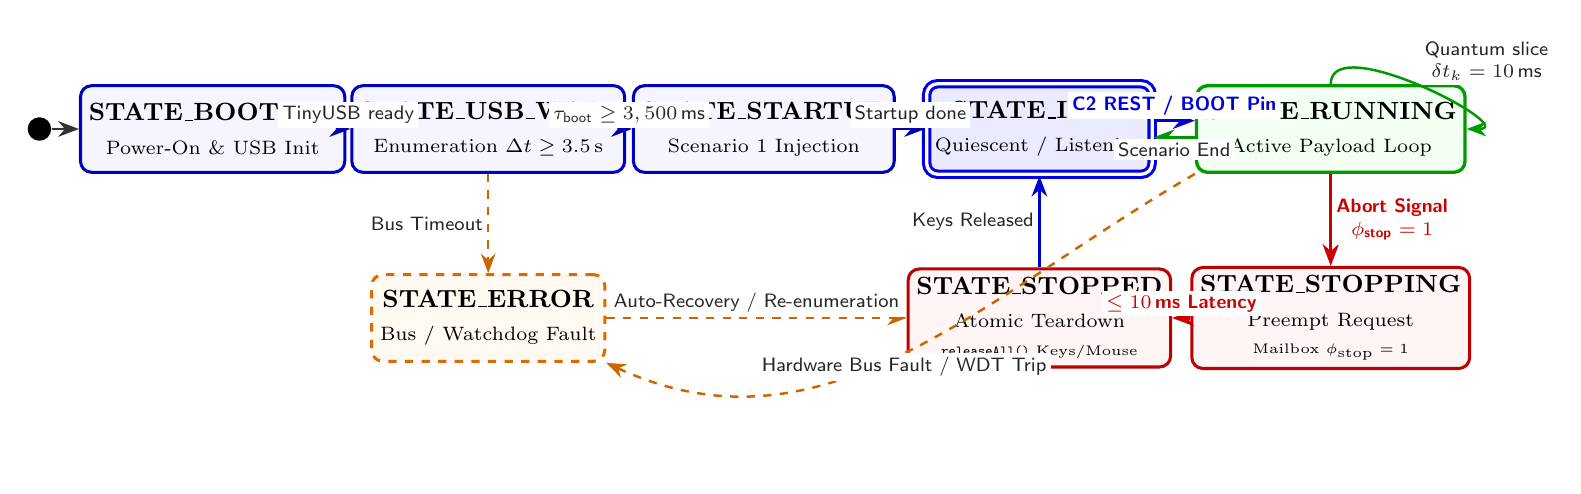
\begin{tikzpicture}[
    >=Stealth,
    node distance=1.8cm,
    font=\small,
    state/.style={
        rectangle,
        rounded corners=4pt,
        draw=blue!75!black,
        line width=1.1pt,
        fill=blue!4!white,
        minimum width=2.4cm,
        minimum height=1.1cm,
        inner sep=3pt,
        align=center
    },
    idle_state/.style={
        rectangle,
        rounded corners=4pt,
        draw=blue!90!black,
        double,
        double distance=1.2pt,
        line width=1.1pt,
        fill=blue!8!white,
        minimum width=2.5cm,
        minimum height=1.15cm,
        inner sep=3pt,
        align=center
    },
    run_state/.style={
        rectangle,
        rounded corners=4pt,
        draw=green!60!black,
        line width=1.2pt,
        fill=green!5!white,
        minimum width=2.5cm,
        minimum height=1.1cm,
        inner sep=3pt,
        align=center
    },
    stop_state/.style={
        rectangle,
        rounded corners=4pt,
        draw=red!75!black,
        line width=1.1pt,
        fill=red!4!white,
        minimum width=2.4cm,
        minimum height=1.1cm,
        inner sep=3pt,
        align=center
    },
    err_state/.style={
        rectangle,
        rounded corners=4pt,
        draw=orange!85!black,
        line width=1.1pt,
        dashed,
        fill=orange!5!white,
        minimum width=2.4cm,
        minimum height=1.1cm,
        inner sep=3pt,
        align=center
    },
    lbl/.style={
        font=\sffamily\scriptsize,
        fill=white,
        inner sep=1.5pt,
        align=center,
        text=black!85
    },
    lbl_red/.style={
        font=\sffamily\scriptsize\bfseries,
        fill=white,
        inner sep=1.5pt,
        align=center,
        text=red!80!black
    },
    lbl_blue/.style={
        font=\sffamily\scriptsize\bfseries,
        fill=white,
        inner sep=1.5pt,
        align=center,
        text=blue!85!black
    }
]

% Start marker
\node[circle, fill=black, inner sep=3pt] (start) at (0, 0) {};

% Top Row: Sequential initialization to IDLE and RUNNING
\node[state] (boot) at (2.2, 0) {\textbf{STATE\_BOOTING}\\[1pt]\scriptsize Power-On \& USB Init};
\node[state] (usbwait) at (5.7, 0) {\textbf{STATE\_USB\_WAIT}\\[1pt]\scriptsize Enumeration $\Delta t \ge 3.5$\,s};
\node[state] (startup) at (9.2, 0) {\textbf{STATE\_STARTUP}\\[1pt]\scriptsize Scenario 1 Injection};
\node[idle_state] (idle) at (12.7, 0) {\textbf{STATE\_IDLE}\\[1pt]\scriptsize Quiescent / Listening};
\node[run_state] (running) at (16.4, 0) {\textbf{STATE\_RUNNING}\\[1pt]\scriptsize Active Payload Loop};

% Bottom Row: Error and Abort Recovery
\node[err_state] (error) at (5.7, -2.4) {\textbf{STATE\_ERROR}\\[1pt]\scriptsize Bus / Watchdog Fault};
\node[stop_state] (stopped) at (12.7, -2.4) {\textbf{STATE\_STOPPED}\\[1pt]\scriptsize Atomic Teardown\\[-1pt]\tiny \texttt{releaseAll()} Keys/Mouse};
\node[stop_state] (stopping) at (16.4, -2.4) {\textbf{STATE\_STOPPING}\\[1pt]\scriptsize Preempt Request\\[-1pt]\tiny Mailbox $\phi_{\text{stop}}=1$};

% Initialization Transitions
\draw[->, line width=1.0pt, draw=black!80] (start) -- (boot);
\draw[->, line width=1.0pt, draw=blue!70!black] (boot) -- node[above, lbl] {TinyUSB ready} (usbwait);
\draw[->, line width=1.0pt, draw=blue!70!black] (usbwait) -- node[above, lbl] {$\tau_{\text{boot}} \ge 3,500$\,ms} (startup);
\draw[->, line width=1.0pt, draw=blue!70!black] (startup) -- node[above, lbl] {Startup done} (idle);

% Operational Loop
\draw[->, line width=1.1pt, draw=blue!80!black] ([yshift=3pt]idle.east) -- node[above, lbl_blue] {C2 REST / BOOT Pin} ([yshift=3pt]running.west);
\draw[->, line width=1.0pt, draw=green!60!black] ([yshift=-3pt]running.west) -- node[below, lbl] {Scenario End} ([yshift=-3pt]idle.east);

% Cooperative slicing self-loop
\draw[->, line width=0.9pt, draw=green!60!black] (running.north) .. controls +(up:0.7cm) and +(right:0.7cm) .. node[above right, lbl] {Quantum slice\\$\delta t_k = 10$\,ms} (running.east);

% Preemption Flow
\draw[->, line width=1.1pt, draw=red!80!black] (running.south) -- node[right, lbl_red] {Abort Signal\\$\phi_{\text{stop}} = 1$} (stopping.north);
\draw[->, line width=1.1pt, draw=red!80!black] (stopping.west) -- node[above, lbl_red] {$\le 10$\,ms Latency} (stopped.east);
\draw[->, line width=1.0pt, draw=blue!80!black] (stopped.north) -- node[left, lbl] {Keys Released} (idle.south);

% Error & Recovery Flow
\draw[->, line width=0.9pt, dashed, draw=orange!80!black] (usbwait.south) -- node[left, lbl] {Bus Timeout} (error.north);
\draw[->, line width=0.9pt, dashed, draw=orange!80!black] (error.east) -- node[above, lbl] {Auto-Recovery / Re-enumeration} (stopped.west);
\draw[->, line width=0.9pt, dashed, draw=orange!80!black] (running.south west) to[out=210, in=-25] node[below, lbl] {Hardware Bus Fault / WDT Trip} (error.south east);

\end{tikzpicture}
\end{document}
